\documentclass[../main-report.tex]{subfiles}
\begin{document}
\section{Giới thiệu}
Trong những năm gần đây, \Gls{blockchain} được biết tới như là công nghệ để vận hành đồng tiền số Bitcoin, số lượng giao dịch và các tài khoản trong mạng Bitcoin đang càng ngày càng tăng cao. Dưới sự phát triển bùng nổ này, không khó để khiến đồng tiền điện tử Bitcoin thu hút được sự chú ý của cộng đồng. \Gls{blockchain} là một cuốn sổ cái mà ở đó các dữ liệu không thể bị chỉnh sửa hoặc xoá khi đã được chấp thuận bởi các nút trong mạng. Vì đặc điểm này nên \gls{blockchain} còn được biết đến như là một công nghệ giúp dữ liệu được lưu trữ toàn vẹn, tin tưởng \cite{yli2016current}. Công nghệ \gls{blockchain} này còn được áp dụng không chỉ về các lĩnh vực tài chính mà nó còn được áp dụng ở một số các lĩnh vực khác như chăm sóc sức khoẻ, sở hữu trí tuệ,\ldots

Chính vì các đặc điểm nổi bật này của \gls{blockchain} mà PwC và VeChain đã tiến hành cuộc khảo sát vào tháng 11 và tháng 12 năm 2017. Kết quả đã chỉ ra rằng hầu hết các doanh nghiệp của họ đang thành lập bộ phận nghiên cứu và phát triển (R\&D) để đầu tư cho \gls{blockchain}. Lý do mà họ (các công ty trong cuộc khảo sát đã triển khai công nghệ \gls{blockchain}) chọn công nghệ này để nghiên cứu và phát triển thì có đến 50\% về lý do bảo mật, các lý do còn lại như phân tán dữ liệu (26.7\%), chứng thực định danh (23.3\%),\ldots

Khóa luận này tập trung vào việc áp dụng công nghệ \gls{blockchain} vào hình thức \glsdesc{crowdfunding} (\Gls{crowdfunding}). Định nghĩa về \gls{crowdfunding} được nhóm tác giả trích từ bài nghiên cứu của tác giả Lambert và Schwienbacher (2010) như sau:

\begin{quote}
\textit{``Crowdfunding  involves  an  open  call,  essentially  through  the Internet, for the provision of financial resources either in form of donationor in exchange for some form of reward and/or voting rights.''} \cite{belleflamme2010crowdfunding}
\end{quote}

Có thể hiểu định nghĩa trên theo tiếng Việt là \gls{crowdfunding} giống như một lời gọi mở, thường được thực hiện qua Internet, để cung cấp nguồn tài chính dưới hình thức tài trợ để đổi lấy phần thưởng hoặc quyền biểu quyết.

\Gls{crowdfunding} là một thị trường chứa hàng tỉ đô-la, những giao dịch quốc tế đã đạt tới 34 tỷ đô-la trong năm 2015, gấp đôi năm trước \cite{hornuf2018economics}. Hiện nay, trên thế giới đã xuất hiện nhiều mô hình gây quỹ cộng đồng có thể kể đến như \textbf{Kickstarter}\footnote{https://www.kickstarter.com} và \textbf{Indiegogo}\footnote{https://www.indiegogo.com}. Những mô hình này cung cấp một platform để cho các chủ đầu tư có thể kêu gọi các nhà đầu tư, đầu tư vào các dự án của họ, các dự án này đa dạng, phong phú về lĩnh vực có thể kể đến như: âm nhạc, sản xuất vật liệu mới, đầu tư về giáo dục hay thậm chí là kêu gọi quỹ từ thiện.

Theo một cuộc nghiên cứu về Kickstarter bắt đầu từ năm 2008 đến tháng 7 năm 2012 của một cuộc điều tra kết quả là có 48.526 nỗ lực kêu gọi dự án với 237 triệu cam kết, và có 23.719 dự án chiếm 48.1\% là kêu gọi quỹ thành công. Kickstarter cũng đã công bố phân tích tổng thể danh sách 26.017 dự án thành công và 33.098 dự án thất bại \cite{mollick2014dynamics}.

Tuy nhiên, các dự án trong Kickstarter đa phần tập trung vào mục đích lợi nhuận, thương mại cụ thể có 16\% về lĩnh vực phim, 13\% liên quan đến âm nhạc, 11\% là về sách và 10\% là các dự án về trò chơi điện tử; còn các dự án phi lợi nhuận, gây quỹ cộng đồng từ thiện chiếm tỉ lệ thấp, hầu như ít xuất hiện trên platform này \footnote{Nguồn: https://thehustle.co/archive/02102019d}. Có thể thấy trên các nền tảng này, nguồn tiền được đóng góp thông qua bên thứ 3 (Visa, Mastercard, \ldots), bên thứ 3 này có tác dụng là nắm giữ nguồn vốn của nhà đầu tư, khi việc gây quỹ thành công, tuỳ vào cơ chế quản lý của nền tảng, nguồn vốn sẽ được xử lý và công nghệ hiện tại mà các platform này sử dụng đều đi qua cơ sở dữ liệu của chính nền tảng đó, điều này đặt ra tính toàn vẹn dữ liệu của dự án cũng như số tiền thật sự mà họ nhận được. Bên cạnh đó, các giải pháp giải quyết rủi ro về vấn đề tính sẵn sàng cao cũng như các cuộc tấn công khác nhằm chiếm đoạt tài sản của các nhà đầu tư chưa được chú ý đến. Tất cả các yếu tố bất lợi trên ta có thể thấy được rằng mô hình gây quỹ cộng đồng truyền thống chưa thật sự an toàn đối với các nhà đầu tư cũng như chủ chiến dịch và đặc biệt là nó chưa quan tâm đến các dự án gây quỹ cộng đồng, phi lợi nhuận. Bằng cách áp dụng blockchain vào mô hình gây quỹ truyền thống, ta có thể loại bỏ các yếu tố bất lợi được đề cập ở trên.
\section{Các nghiên cứu liên quan}
\label{sec:related-work}
Với ý tưởng áp dụng \gls{blockchain} vào các chiến dịch với mục đích phi lợi nhuận – trên thế giới đã có một chiến dịch có tên là \textbf{Usizo}\footnote{http://secret.usizo.org}, dự án này nhằm mục đích mua điện cho trường học ở miền nam của châu Phi bằng Bitcoin  được đề xuất bởi Nir Kshetri – một giáo sư tại trường đại học North Carolina, ý tưởng của chiến dịch này đó chính là áp dụng đồng tiền kỹ thuật số Bitcoin từ các nhà tài trợ để thanh toán tiền điện cho trường học, số tiền được nhận sẽ được thanh toán trực tiếp vào nguồn điện mà nhà trường đã sử dụng \cite{goranovic2017blockchain}. Theo đó, các nhà tài trợ có thể theo dõi số lượng nguồn điện mà nhà trường tiêu thụ và đồng thời tính toán nguồn tiền đóng góp của họ.

Trong một bài báo của tác giả Nazmus Saadat \cite{saadat2019blockchain} đề xuất mô hình gây quỹ cộng đồng áp dụng hợp đồng thông minh trên nền tảng Ethereum \gls{blockchain} để các hợp đồng được thực hiện hoàn toàn tự động, do đó ngăn ngừa gian lận và đảm bảo rằng các dự án có thể được phân phối trong thời gian nhất định. Hợp đồng thông minh sẽ giữ tiền của người đóng góp cho tới khi đạt được mục tiêu đặt ra. Tùy thuộc vào kết quả gây quỹ, tiền sẽ được trao cho chủ dự án hoặc trả lại an toàn cho người đóng góp. Tuy nhiên trong quy trình tạo chiến dịch ở hình \ref{fig:crowdfunding-proccess-old}, người tạo chiến dịch không được xác minh danh tính trước khi tạo chiến dịch, mà chỉ đơn thuần là đăng nhập vào một trình quản lý ví ethereum được gọi là Metamask\footnote{https://metamask.io}. Mà trên ví Metamask không cung cấp bất kì cơ chế nào để định danh người dùng.

\begin{figure}[ht!]
\begin{center}
\label{fig:crowdfunding-proccess-old}
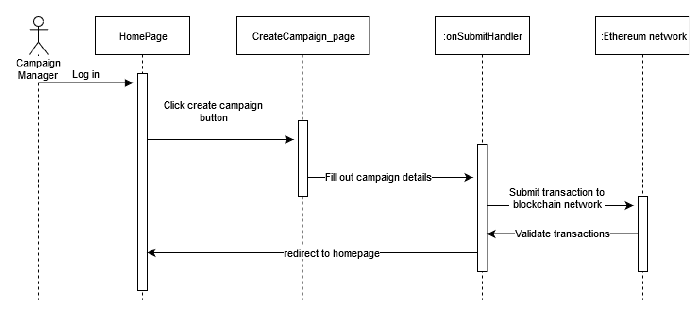
\includegraphics[scale=0.8]{crowdfunding-process-old}
\caption{Sơ đồ quy trình tạo chiến dịch trong mô hình của tác giả Nazmus Saadat}
\end{center}
\end{figure}

Một hệ thống khác cũng ứng dụng hợp đồng thông minh trên nền tảng Ethereum được gọi là \textbf{WeiFund}\footnote{http://weifund.io}, tuy nhiên trong quy trình hoàn tiền cho người đóng góp khi mục tiêu gây quỹ thất bại được thực hiện một cách thủ công, tức người đóng góp phải thực hiện nhấp chuột vào một nút được gọi là ``Claim Refund Owed'' thì tiền mới được hoàn lại.

Một ứng dụng gây quỹ cộng đồng cho mục đích từ thiện khác được tổ chức có tên \textbf{\acrfull{bcf}}\footnote{https://www.binance.charity} thực hiện. Tuy nhiên việc đăng kí chiến dịch trên hệ thống của BCF hoàn toàn chưa có tính mở, chưa cho phép cộng đồng đăng kí chiến dịch.

\section{Kiến thức nền tảng}
\subsection{Công nghệ blockchain}

\subsection{Nền tảng Ethereum}

\subsection{Hợp đồng thông minh - Smart contract}

\end{document}